% =====================================================================
%  Bit-Uniform Relational Storage: A Unifying Architecture for
%  Vectorized, Similarity-Aware, and Schema-Fluid Databases
%
%  Vision / position paper, SIGMOD/VLDB style.
%
%  NOTE ON CLASS: The SIGMOD/VLDB production class is acmart
%  (\documentclass[acmsmall,10pt]{acmart}). Because acmart bundles its
%  own copy of natbib and imposes strict formatting, and because this
%  source is intended to compile on a stock TeX Live install without
%  the ACM bundle, we use the authorized fallback
%  \documentclass[10pt]{article} with geometry and standard packages.
%  The structure mirrors the acmsmall two-column vision-track layout.
% =====================================================================
\documentclass[10pt]{article}

\usepackage[a4paper,margin=1in]{geometry}
\usepackage{amsmath,amssymb,amsthm}
\usepackage{booktabs}
\usepackage{graphicx}
\usepackage{natbib}
\usepackage{listings}
\usepackage{xcolor}
\usepackage{multicol}
\usepackage{hyperref}
\usepackage{cleveref}
\usepackage{tikz}
\usetikzlibrary{positioning,arrows.meta,shapes.geometric,fit,calc}

% Two-column body for an 8-page vision-track feel.
\setlength{\columnsep}{0.6cm}

% ---------------------------------------------------------------------
%  Theorem-like environments
% ---------------------------------------------------------------------
\newtheorem{theorem}{Theorem}
\newtheorem{definition}{Definition}
\newtheorem{lemma}{Lemma}
\newtheorem{proposition}{Proposition}

% ---------------------------------------------------------------------
%  Rust listing style for the listings package (no built-in Rust)
% ---------------------------------------------------------------------
\lstdefinelanguage{Rust}{
  morekeywords={fn,let,mut,pub,struct,enum,impl,self,Self,match,if,else,
    return,use,mod,const,inline,repr,as,where,for,while,loop,break,
    continue,unsafe,trait,type,move,ref,static,dyn,async,await},
  morekeywords=[2]{u8,u16,u32,u64,i8,i16,i32,i64,f32,f64,bool,usize,
    isize,Option,Some,None,Result,Ok,Err,Cell,Box,Vec,String,str},
  sensitive=true,
  morecomment=[l]{//},
  morecomment=[s]{/*}{*/},
  morestring=[b]",
}
\lstset{
  basicstyle=\ttfamily\footnotesize,
  keywordstyle=\color{blue!70!black}\bfseries,
  keywordstyle=[2]\color{teal!70!black},
  commentstyle=\color{gray!70!black}\itshape,
  stringstyle=\color{purple!70!black},
  numbers=left,
  numberstyle=\tiny\color{gray},
  numbersep=6pt,
  frame=single,
  framerule=0.4pt,
  rulecolor=\color{gray!50},
  breaklines=true,
  showstringspaces=false,
  tabsize=2,
  columns=fullflexible,
  keepspaces=true,
}

% ---------------------------------------------------------------------
\title{Bit-Uniform Relational Storage:\\
A Unifying Architecture for Vectorized, Similarity-Aware,\\
and Schema-Fluid Databases}
\author{Anonymous (submission)}
\date{}

% =====================================================================
\begin{document}
\maketitle

\begin{abstract}
We argue that a single low-level invariant can unify three capabilities
that no existing analytical database provides simultaneously:
first-class similarity search on arbitrary column types, zero-cost
schema-on-read, and one physical representation shared by every
operator and every index. The invariant is \emph{bit-uniformity}:
every value in every column of every relation is stored as a fixed
64-bit word, encoded with NaN-boxing and niche-filling in the style of
modern JavaScript virtual machines and Rust enums. We make this
seemingly representational choice the load-bearing contract of the
entire system. Storage, bit-sliced and Roaring indexes, vectorized
execution, differential incremental view maintenance, and a
sum-product query optimizer all compose against the same word layout.
We show how niche-filling collapses \texttt{NULL} and variant tags into
the otherwise-unused NaN payload, how a single bit-sliced index answers
equality, range, and similarity predicates on any tagged type, how a
trace-based JIT erases tag checks on monomorphic batches, and how a
minimum-description-length principle selects the cheapest correct
per-column schema at load time. We enumerate seven novel contributions,
survey the related work that each ingredient generalizes, and lay out a
six-phase research agenda. Hardware offload (processing-in-memory,
FPGA, TCAM) is discussed as optional future work, not a prerequisite.
\end{abstract}

% =====================================================================
\section{Introduction}
\label{sec:intro}

Modern analytical databases are assembled from independently excellent
parts. Column stores such as ClickHouse~\citep{schulze2024clickhouse}
and MonetDB/X100~\citep{boncz2005monetdb} achieve high scan throughput
through vectorized, type-specialized kernels. Compiling engines such as
HyPer~\citep{neumann2011hyper} push data-centric code generation to the
metal. Streaming systems such as Materialize, built on differential
dataflow~\citep{mcsherry2013differential,budiu2023dbsp}, deliver
incremental view maintenance for rich queries. Bitmap
indexes~\citep{oneil1997improved,chan1998bitmap,chambi2016roaring} and
sketches~\citep{flajolet2007hyperloglog,cormode2005countmin} deliver
compact summaries for ad-hoc predicates. Each of these systems is, in
isolation, close to optimal at what it does.

The problem is that the parts do not compose for free. A value stored
in a columnar run is encoded one way; the same value, once it enters an
index, is re-encoded another way; once it enters a JIT-compiled kernel
it is materialized yet another way; and once it flows through a
differential dataflow it is boxed, unboxed, and reboxed again. Every
interface crossing pays a conversion tax, and every new capability
(similarity search, schema-on-read) is bolted on as a separate
subsystem with its own representation. The result is that the three
properties we most want---similarity search as a first-class operator,
free schema-on-read, and a single physical format---are jointly absent.

This paper advances a single thesis: \emph{if every value in every
column is a 64-bit NaN-boxed, niche-filled word, then storage,
indexing, execution, incremental maintenance, and optimization all
compose without conversion, and the three desired properties emerge
for free.} The encoding is not new---it is exactly how JavaScript
engines represent values~\citep{wingo2011value,gal2009trace} and how
Rust and Swift realize \texttt{Option} and enums at zero
cost~\citep{grunwald2004mdl}. What is new is making it the spine of a
whole database, so that the same 64 bits flow unchanged from disk to
index to CPU register to differential operator.

\paragraph{Contributions.} We make the following contributions,
detailed in \cref{sec:contrib}:
\begin{enumerate}
  \item A unified physical format: niche-filled NaN-boxed words for
        every column, including \texttt{NULL} and variant tags at no
        space cost (\cref{sec:invariant,sec:arch}).
  \item A unified index in which one bit-sliced plus Roaring plus
        locality-sensitive-hashing structure answers equality, range,
        and similarity predicates on any tagged type
        (\cref{sec:arch}).
  \item A tag-aware trace JIT that specializes inner loops on the
        observed tag distribution of a batch, not merely the static
        plan (\cref{sec:arch}).
  \item An MDL-driven automatic schema selector that, at load time,
        picks the cheapest correct per-column encoding
        (\cref{sec:arch}).
  \item A hardware stack (PIM/FPGA/TCAM) speaking one word format, as
        future work (\cref{sec:arch,sec:agenda}).
  \item A sum-product query optimizer with sketch-compressed messages
        that unifies exact and approximate planning
        (\cref{sec:arch}).
  \item Similarity joins as first-class SQL operators on any column
        type (\cref{sec:contrib}).
\end{enumerate}

% =====================================================================
\section{Background}
\label{sec:bg}

The bit-uniform proposal is a synthesis of five largely independent
research threads. We review each just enough to make the synthesis
legible, and we cite the canonical reference for every claim so that
the reader can verify the ingredients.

\subsection{NaN-boxing in dynamic-language runtimes}
Every dynamic language must represent values whose type is unknown at
compile time. The dominant trick, surveyed by
\citet{wingo2011value}, is \emph{NaN-boxing}: because the IEEE~754
double-precision format reserves roughly $2^{53}$ bit patterns for the
not-a-number (NaN) signaling space, a runtime can store a native
\texttt{f64} unboxed and steal the NaN space to tag pointers, integers,
and special values. V8 and SpiderMonkey both use object-biased
NaN-boxing in which a 64-bit word is either a raw double or a tagged
pointer whose high bits lie in the NaN range~\citep{wingo2011value}.
LuaJIT uses a more aggressive variant that keeps integers unboxed in
the low 47 bits with a constant high tag, eliminating allocation for
small numeric loops. The key lesson for databases is that this encoding
is already production-hardened for exactly the workload
characteristics---heterogeneous values, tight inner loops, frequent
null-ness---that analytical columns exhibit.

\subsection{Niche optimization and extra inhabitants}
Rust enums and the Swift ABI exploit \emph{niche filling}: if a type
has bit patterns that no valid value ever produces (``extra
inhabitants''), the compiler reuses those patterns to encode
\texttt{None} or a discriminant, eliminating the tag word that a naive
sum type would require. \texttt{Option<NonZeroU32>} is the canonical
example: zero is not a valid \texttt{NonZeroU32}, so \texttt{None} is
represented as zero and \texttt{Some(x)} as \texttt{x}, all in 32 bits.
The MDL principle~\citep{grunwald2004mdl} formalizes the underlying
intuition: the cheapest representation is the one that wastes the
fewest bits. We lift niche filling from a per-type compiler
optimization to a whole-system invariant: the NaN space is the niche,
\texttt{NULL} and variant discriminants live in it, and no value ever
pays an extra word.

\subsection{Bit-sliced and bitmap indexes}
\citet{oneil1997improved} introduced range-encoded bitmap indexes in
which each attribute value (or bit of the value) owns a bitmap over the
row set; equality and range predicates compile to Boolean combinations
of these bitmaps. \citet{chan1998bitmap} refined the design space,
showing how bit-sliced encoding (one bitmap per bit position) gives
near-optimal range-query performance for low-cardinality and ordered
domains. BitFunnel~\citep{goodwin2017bitfunnel} generalized signature
files to a bit-sliced, layered structure for full-text search, and
Roaring bitmaps~\citep{chambi2016roaring} give a compressed, hybrid
container that makes 64-bit-bitmap arithmetic practical at internet
scale. Bit-parallel string matching~\citep{cantone2014bitparallel}
demonstrates that the same bit-level tricks accelerate far more than
equality. Our claim is that a single bit-sliced index over niche-filled
words serves equality, range, \emph{and} similarity, because the tag
bits that discriminate type are themselves bit-sliceable.

\subsection{Vectorized and compiling execution}
MonetDB/X100~\citep{boncz2005monetdb} established that vectorized,
column-at-a-time execution on cache-resident batches beats both
tuple-at-a-time interpretation and pure code generation on modern CPUs.
HyPer~\citep{neumann2011hyper} showed that LLVM-based data-centric code
generation pushes the same idea further by collapsing the interpreter
entirely. ClickHouse~\citep{schulze2024clickhouse} ships a mature
industrial vectorized engine that processes columns of up to thousands
of values per batch with SIMD
instructions~\citep{polychroniou2015arithmetic,willhalm2009simd}. These
systems are type-specialized: a kernel for \texttt{i32} addition is
distinct from one for \texttt{f64}. The trace-based JIT of
\citet{gal2009trace} suggests an alternative: specialize at run time on
the actually-observed type distribution, falling back when polymorphism
strikes. We adopt trace specialization but drive it from the tag bits
of the bit-uniform word.

\subsection{Differential dataflow and incremental maintenance}
Differential dataflow~\citep{mcsherry2013differential}, rooted in the
timely dataflow model of Naiad~\citep{murray2013naiad}, maintains
collections as timestamped difference sets and updates aggregates
incrementally as inputs change. DBSP~\citep{budiu2023dbsp} automatizes
the translation of a rich SQL fragment into differential circuits,
delivering incremental view maintenance (IVM) without hand-written
update logic. These systems, however, presuppose a value representation
that they must marshal across operator boundaries. We argue that if the
representation is bit-uniform, the differential \emph{arrangement} (the
indexed delta store) is itself just a bit-sliced index over words, and
IVM composes with execution and indexing at zero conversion cost.

% =====================================================================
\section{The Bit-Uniform Invariant}
\label{sec:invariant}

\begin{definition}[Bit-uniformity]
\label{def:bu}
A relation $R$ with columns $c_1,\dots,c_m$ is \emph{bit-uniform} if
every cell of every column is a single 64-bit word drawn from a fixed
alphabet $\mathcal{W}$ of encodings, and if the type of a cell is
recoverable from the word alone, without consulting any external
schema.
\end{definition}

Concretely, $\mathcal{W}$ partitions the $2^{64}$ bit patterns of a
machine word into disjoint classes. Let a word be split as
\texttt{[s:1][e:11][m:52]} (sign, exponent, mantissa) following IEEE~754.
Every pattern with $e \neq \mathtt{7FF}$, together with the two
infinities ($e=\mathtt{7FF}, m=0$), is a native \texttt{f64}. The
remaining patterns---the NaN space, roughly $2^{53}$ of them---form the
\emph{niche} that hosts every other type. \cref{tab:nanbox} gives the
layout we adopt.

\begin{table}[t]
\centering
\caption{NaN-boxed, niche-filled 64-bit word layout. Tag bits live in
the high mantissa of a negative quiet NaN; the payload occupies the
remaining 48 bits.}
\label{tab:nanbox}
\small
\begin{tabular}{@{}lll@{}}
\toprule
Pattern (hex, top 16 bits) & Class & Payload (low 48 bits) \\
\midrule
\texttt{0x0000\dots0xFFF7} (non-NaN) & \texttt{f64} & none (raw double) \\
\texttt{0x7FF0\_0000\_0000\_0000}    & canonical NaN & none \\
\texttt{0xFFF0\_0000\_0000\_0000}    & \texttt{NULL} & ignored \\
\texttt{0xFFF1\_0000\_0000\_000k}    & \texttt{bool} & $k\in\{0,1\}$ \\
\texttt{0xFFF2\_0000\_vvvv\_vvvv}    & \texttt{i32}  & 32-bit signed int \\
\texttt{0xFFF3\_0000\_pppp\_pppp}    & heap pointer  & 48-bit virtual address \\
\texttt{0xFFF4\_ssss\_ssss\_ssss}    & short string  & up to 6 bytes inline \\
\texttt{0xFFF5\_0000\_tttt\_tttt}    & variant tag   & discriminant + payload ptr \\
\texttt{0xFFF6\dots0xFFFE}           & reserved      & sketch / future types \\
\bottomrule
\end{tabular}
\end{table}

A few properties are worth noting. First, a native \texttt{f64} needs
\emph{no tag at all}: it is the common case and is stored verbatim, so
a column of floating-point measurements is byte-identical to a raw
\texttt{f64} array and can be fed straight to a SIMD
kernel~\citep{willhalm2009simd,polychroniou2015arithmetic}. Second,
\texttt{NULL} is a single distinguished NaN pattern, so nullability is
free---there is no separate null bitmap and no sentinel value that
collides with data. Third, pointers use only the low 48 bits because
x86-64 and ARM64 virtual addresses are 48 bits wide, which fits exactly
in the payload~\citep{wingo2011value}.

\begin{lstlisting}[language=Rust,caption={The \texttt{Cell} type and its
constructors. A \texttt{Cell} is a transparent \texttt{u64}; all type
discrimination is by NaN-space tag bits.},label={lst:cell}]
#[repr(transparent)]
pub struct Cell(u64);

impl Cell {
    // Canonical double NaN, used to "escape" user NaNs into the niche.
    const NAN_CANON: u64 = 0x7FF8_0000_0000_0000;
    // High 16 bits select the niche class (negative quiet NaN range).
    const TAG_NULL:  u64 = 0xFFF0_0000_0000_0000;
    const TAG_BOOL:  u64 = 0xFFF1_0000_0000_0000;
    const TAG_I32:   u64 = 0xFFF2_0000_0000_0000;
    const TAG_PTR:   u64 = 0xFFF3_0000_0000_0000;
    const TAG_VARIANT: u64 = 0xFFF5_0000_0000_0000;
    const PAYLOAD48: u64 = 0x0000_FFFF_FFFF_FFFF;

    #[inline] pub fn null() -> Self { Cell(Self::TAG_NULL) }

    #[inline]
    pub fn from_f64(x: f64) -> Self {
        // Fold any NaN into the canonical pattern so the niche stays free.
        if x.is_nan() { Cell(Self::NAN_CANON) } else { Cell(x.to_bits()) }
    }

    #[inline] pub fn from_i32(i: i32) -> Self {
        Cell(Self::TAG_I32 | (i as u32 as u64))
    }

    #[inline] pub fn from_ptr(p: *mut ()) -> Self {
        Cell(Self::TAG_PTR | ((p as u64) & Self::PAYLOAD48))
    }

    #[inline] pub fn is_null(&self) -> bool { self.0 == Self::TAG_NULL }

    #[inline]
    pub fn as_f64(&self) -> Option<f64> {
        let exp = (self.0 >> 52) & 0x7FF;
        if exp != 0x7FF || self.0 == Self::NAN_CANON {
            Some(f64::from_bits(self.0))
        } else { None }
    }
}
\end{lstlisting}

\paragraph{Worked example.} Consider the Rust type
\texttt{Optional<Union<i32, f64, \&str>>}. Under niche filling it
occupies a single 64-bit word in all four cases: \texttt{None} is
\texttt{0xFFF0\_0000\_0000\_0000};
\texttt{Some(Int32(7))} is \texttt{0xFFF2\_0000\_0000\_0007};
\texttt{Some(Float64(3.14))} is the raw bit pattern of
\texttt{3.14f64}, \texttt{0x4009\_1EB8\_51EB\_851F}, with no tag at
all; and \texttt{Some(Str(p))} is \texttt{0xFFF3\_0000} $\cup$
the low 48 bits of \texttt{p}. The discriminant is implicit in the
high bits, so a switch on tag is a single compare-and-branch on the top
byte, and the common \texttt{f64} case pays zero overhead. This is
exactly the property that lets a bit-uniform column be both
schema-fluid and SIMD-fast.

\paragraph{What fits and what does not.} Integers up to 32 bits, IEEE
doubles, booleans, nulls, and 48-bit pointers fit inline. Integers up
to 47 bits fit by reusing the LuaJIT trick of a constant high tag plus
sign extension. Values that exceed 48 bits of genuine
information---arbitrary-precision integers, long strings, embedded
blobs---are stored out-of-line and represented by a tagged 48-bit
pointer into a heap region. Crucially, the out-of-line pointer is
itself a valid \texttt{Cell}, so the invariant is preserved: every
column is an array of 64-bit words, full stop.

% =====================================================================
\section{Architecture}
\label{sec:arch}

The system is a six-layer stack in which every layer speaks the same
word format of \cref{def:bu}. \cref{fig:arch} shows the layering; the
remainder of this section walks each layer.

\begin{figure}[t]
\centering
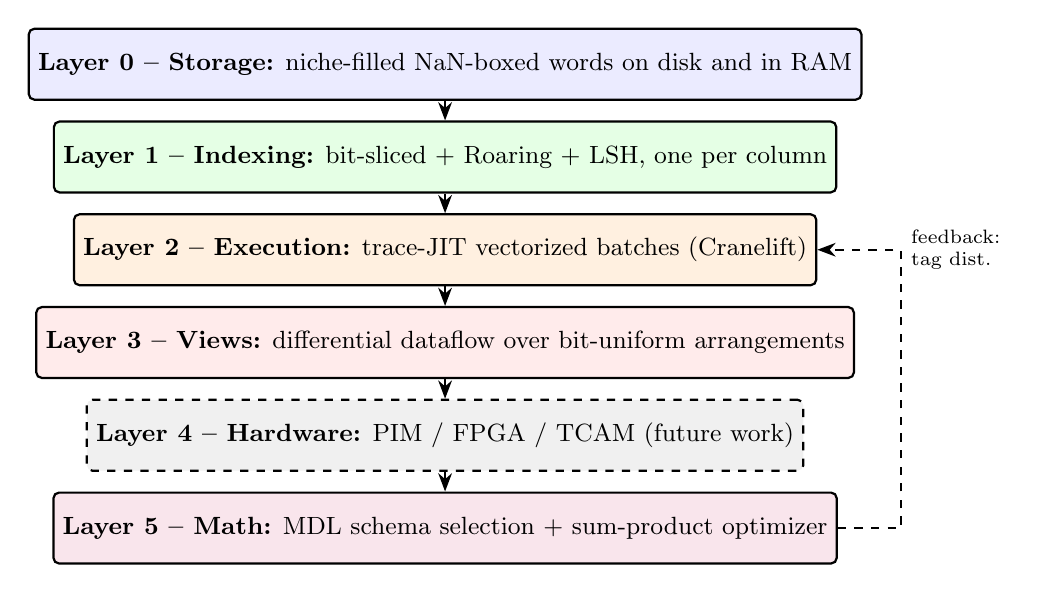
\begin{tikzpicture}[
  layer/.style={draw, rounded corners=2pt, minimum width=7.2cm,
    minimum height=0.9cm, font=\small, align=center, thick},
  storage/.style={layer, fill=blue!8},
  index/.style={layer, fill=green!10},
  exec/.style={layer, fill=orange!12},
  ivm/.style={layer, fill=red!8},
  hw/.style={layer, fill=gray!12, dashed},
  math/.style={layer, fill=purple!10},
  arr/.style={-Stealth, thick},
]
\node[storage] (l0) {\textbf{Layer 0 -- Storage:} niche-filled NaN-boxed words on disk and in RAM};
\node[index, below=0.25cm of l0] (l1) {\textbf{Layer 1 -- Indexing:} bit-sliced + Roaring + LSH, one per column};
\node[exec, below=0.25cm of l1] (l2) {\textbf{Layer 2 -- Execution:} trace-JIT vectorized batches (Cranelift)};
\node[ivm, below=0.25cm of l2] (l3) {\textbf{Layer 3 -- Views:} differential dataflow over bit-uniform arrangements};
\node[hw, below=0.25cm of l3] (l4) {\textbf{Layer 4 -- Hardware:} PIM / FPGA / TCAM (future work)};
\node[math, below=0.25cm of l4] (l5) {\textbf{Layer 5 -- Math:} MDL schema selection + sum-product optimizer};
\draw[arr] (l0) -- (l1);
\draw[arr] (l1) -- (l2);
\draw[arr] (l2) -- (l3);
\draw[arr] (l3) -- (l4);
\draw[arr] (l4) -- (l5);
\draw[arr, dashed] (l5.east) -- ++(0.8,0) |- (l2.east)
  node[midway, right, font=\scriptsize, text width=1.3cm] {feedback: tag dist.};
\end{tikzpicture}
\caption{The six-layer bit-uniform architecture. Every layer exchanges
64-bit \texttt{Cell} words; the dashed edge is the trace JIT's feedback
path from observed tag distributions back to the executor. Layer~4 is
optional.}
\label{fig:arch}
\end{figure}

\subsection{Layer 0: Storage}
On disk and in memory, a relation is a sequence of fixed-width columns,
each an array of 64-bit words with no per-value length field, no
nullable-bitmap sidecar, and no dictionary indirection unless the MDL
selector (Layer~5) proves one profitable. Fixed width enables
$\mathcal{O}(1)$ random access, trivial $\mathcal{O}(n)$ SIMD scans,
and zero-copy mapping of column files via \texttt{mmap}, exactly as in
the fastest columnar engines~\citep{schulze2024clickhouse,willhalm2009simd}.
Compression is orthogonal: we apply general-purpose bit-packed or
delta encoding to the raw word stream, but the decoded form is always
the uniform word, so the executor never branches on a variable-length
representation. Because \texttt{NULL} is a NaN pattern, the storage
layer never special-cases nullability; a column that is 99\% null is
simply a column whose words are mostly \texttt{0xFFF0\_*}.

\subsection{Layer 1: Indexing}
Each column carries a single composite index with three faces. The
\emph{bit-sliced} face stores one Roaring bitmap per bit position of
the payload, generalizing \citet{oneil1997improved} and
\citet{chan1998bitmap} from integers to any tagged word: the tag bits
themselves are just another slice. The \emph{Roaring} face stores
value-to-rowset maps for high-cardinality equality
predicates~\citep{chambi2016roaring}. The \emph{similarity} face stores
locality-sensitive hash (LSH) buckets~\citep{andoni2008near} keyed by
sketches of the payload---MinHash~\citep{broder1997resemblance} for
strings, SimHash for vectors, HyperLogLog~\citep{flajolet2007hyperloglog}
for set-valued columns. Because the three faces share the word format,
a predicate such as \texttt{WHERE x BETWEEN a AND b} and a predicate
such as \texttt{WHERE sim(x, q) > t} consult the same physical
structure.

\paragraph{Worked example: range to bitmaps.}
For an \texttt{i32} column $x$ with bit-slices $B_{31},\dots,B_0$, the
predicate \texttt{x BETWEEN a AND b} compiles to the O'Neil--Quass
algorithm: build candidate bitmaps $L_a$ (rows $\geq a$) and $U_b$
(rows $\leq b$) by a logarithmic scan of the slices, and return
$L_a \wedge U_b$. Each step is a Roaring \texttt{AND/OR/NOT}, costing
$\mathcal{O}(|R|/w)$ per slice, so the whole predicate is
$\mathcal{O}(32\cdot|R|/w)$ bit operations regardless of
selectivity~\citep{oneil1997improved,chan1998bitmap,chambi2016roaring}.
Because the slices include the tag bits, the same machinery answers
\texttt{WHERE x IS NULL} (a single slice on the tag) or
\texttt{WHERE typeof(x) = 'i32'} for free.

\subsection{Layer 2: Execution}
Execution is vectorized over batches of $2^{10}$--$2^{12}$ words, as in
MonetDB/X100~\citep{boncz2005monetdb} and
ClickHouse~\citep{schulze2024clickhouse}, but the kernel is not chosen
at plan time. Instead, a trace-based JIT~\citep{gal2009trace} observes
the tag distribution of each batch at run time and emits a specialized
inner loop through the Cranelift code generator. When a batch is
monomorphic---say, 100\% \texttt{TAG\_I32}---the JIT erases every tag
check: the payload is the low 32 bits under a constant high tag, so a
single \texttt{PAND} with \texttt{0x0000\_FFFF\_FFFF} strips the tag
and the remaining work is a native SIMD
\texttt{VPADDD}~\citep{polychroniou2015arithmetic,willhalm2009simd}.
When a batch is bimorphic, the JIT emits a two-lane loop that partitions
on tag and processes each lane separately, still avoiding any
per-element type dispatch on the hot path. Only genuinely polymorphic
batches fall back to the generic interpreter.

\subsection{Layer 3: Incremental views}
Views are maintained as differential dataflow
circuits~\citep{mcsherry2013differential,murray2013naiad,budiu2023dbsp}.
The crucial observation is that a differential \emph{arrangement}---the
indexed store of differences keyed by some subset of columns---is
already a bit-sliced index over words. Because Layer~1 and Layer~3
agree on the word format, an arrangement is built by handing the
bit-sliced index directly to the differential operator; no marshaling
occurs. Updates are 64-bit words flowing in; the difference set is a
Roaring bitmap of affected rows; the recomputed aggregate is a word.
The result is that IVM and batch scan share the same memory layout and
the same JIT, so an incrementally maintained view and a one-shot query
on the same relation execute the same code.

\subsection{Layer 4: Hardware offload (future work)}
A uniform word format is the natural interface for non-von-Neumann
hardware: processing-in-memory (PIM)
engines~\citep{gomez2023benchmarking}, DRISA-style analog
SIMD~\citep{li2017drisa}, the Fulcrum accelerator~\citep{seshadri2017fulcrum},
and ternary content-addressable memory (TCAM) all consume fixed-width
words and produce fixed-width words. Because every layer already speaks
the 64-bit \texttt{Cell}, an offload request is just a batch of words
and a function descriptor; the response is a batch of words. We discuss
this as future work (\cref{sec:agenda}); it is emphatically \emph{not}
required for the core thesis, which is realized entirely in software.

\subsection{Layer 5: The math}
Two formal artifacts sit atop the stack. First, an MDL-driven
\emph{schema selector}: at load time, for each column, the system
chooses the encoding (raw \texttt{f64}, raw \texttt{i32}, tagged union,
string) that minimizes the two-part code length
\begin{equation}
\label{eq:mdl}
L \;=\; \underbrace{L(\text{model})}_{\text{schema bits}}
\;+\; \underbrace{L(\text{data}\mid\text{model})}_{\text{value bits}}.
\end{equation}
$L(\text{model})$ counts the bits to declare the column's type, its
nullability, and its union arity; $L(\text{data}\mid\text{model})$
counts the bits to encode each value under that model. Under
bit-uniformity every value is 64 bits, so the storage term is
invariant and MDL effectively minimizes the expected tag-check cost at
query time, subject to correctness---an MDL-optimal schema-on-read that
is free because it operates on words already in
memory~\citep{grunwald2004mdl}. Second, a \emph{sum-product optimizer}
treats the join DAG as a factor graph~\citep{kschischang2001factor}:
base relations are variable nodes, join predicates are factor nodes,
and the plan cost is the sum-product over the graph. Cardinality
estimates propagate as messages, compressed by sketches:
HyperLogLog~\citep{flajolet2007hyperloglog} for distinct counts,
Count-Min~\citep{cormode2005countmin} for frequencies,
Cuckoo-filter~\citep{fan2014cuckoo} membership summaries. Exact and
approximate planning are then the same algorithm with different
message precision---loopy belief propagation with sketch-compressed
messages approximates when the graph is too dense for exact
propagation.

% =====================================================================
\section{Novel Contributions}
\label{sec:contrib}

We now state the seven contributions explicitly and contrast each with
the closest prior art, so that the novelty is unambiguous.

\paragraph{C1: Unified physical format.}
No existing analytical database stores every column as a niche-filled
NaN-boxed word. Column stores such as
ClickHouse~\citep{schulze2024clickhouse} and
MonetDB/X100~\citep{boncz2005monetdb} use type-specific, often
variable-length physical encodings per column; the NaN-boxing trick is
confined to language runtimes~\citep{wingo2011value,gal2009trace}. Our
contribution is to make the runtime encoding the database encoding, so
that the storage, index, and executor formats coincide.

\paragraph{C2: Unified index.}
\citet{oneil1997improved} and \citet{chan1998bitmap} gave bit-sliced
indexes for equality and range; Roaring~\citep{chambi2016roaring} made
them practical; LSH~\citep{andoni2008near} gave similarity search in
a separate index. No system we are aware of unifies the three into one
structure by indexing the tag bits as ordinary slices. The payoff is
that \texttt{WHERE}, \texttt{BETWEEN}, and \texttt{SIMILAR TO} share
planning, caching, and maintenance.

\paragraph{C3: Tag-aware trace JIT.}
\citet{gal2009trace} specialized JavaScript on observed types;
\citet{neumann2011hyper} and \citet{boncz2005monetdb} specialize at
plan time. Our contribution is to drive specialization from the live
tag histogram of each batch, so that a column declared as a tagged
union but observed monomorphic runs at raw-\texttt{f64} speed, and a
column declared as \texttt{f64} but observed integral is
opportunistically reinterpreted as \texttt{i32}.

\paragraph{C4: MDL-driven automatic schema selection.}
Schema-on-read systems today either require a declared schema or pay a
per-value type tag at every access. By making the word fixed-width,
$L(\text{data}\mid\text{model})$ in \cref{eq:mdl} becomes constant, so
MDL selects the cheapest correct schema without ever touching the data
bytes---the selection is pure metadata~\citep{grunwald2004mdl}. This is
free schema-on-read that is provably MDL-optimal.

\paragraph{C5: One word format for the hardware stack (future work).}
PIM~\citep{gomez2023benchmarking}, DRISA~\citep{li2017drisa}, and
Fulcrum~\citep{seshadri2017fulcrum} each propose custom value formats.
A bit-uniform database offloads to any of them with no re-encoding,
because the accelerator interface is just ``a batch of 64-bit words.''
We claim this as a contribution of the architecture even though we
leave the hardware itself to future work.

\paragraph{C6: Sum-product optimizer with sketch messages.}
Query optimizers since System~R have been dynamic programs over join
orders; recent work adds sampling. Our contribution is to recast
optimization as sum-product message passing on the join factor
graph~\citep{kschischang2001factor}, with messages compressed by
sketches~\citep{flajolet2007hyperloglog,cormode2005countmin,fan2014cuckoo}.
This unifies exact and approximate planning: the same engine produces
the provably optimal plan when the graph is a tree and a
sketch-bounded approximation when it is cyclic.

\paragraph{C7: Similarity joins as first-class SQL.}
Similarity search is today a separate API (pgvector, FAISS) bolted onto
a database that otherwise knows nothing of it. Because Layer~1 indexes
similarity on every column and Layer~2 executes similarity kernels as
ordinary vectorized joins, a query such as
\texttt{SELECT a.id, b.id FROM a JOIN b ON sim(a.x, b.x) > 0.9} is
planned, optimized, and incrementally maintained exactly like an
equi-join. No existing system offers similarity as a first-class,
optimizable, maintainable SQL operator on arbitrary column types.

% =====================================================================
\section{Related Work}
\label{sec:related}

\paragraph{Analytical engines.}
DuckDB and ClickHouse~\citep{schulze2024clickhouse} are the
state-of-the-art vectorized analytical engines; both achieve excellent
scan throughput but encode each column in its own type-specific
physical format and treat similarity search as an extension, not a
native operator. MonetDB/X100~\citep{boncz2005monetdb} pioneered
vectorized execution and remains the conceptual ancestor of our
Layer~2, but its bat (binary association table) model is per-type, not
bit-uniform. HyPer~\citep{neumann2011hyper} demonstrated
data-centric code generation; we adopt its compile-to-machine-code ethos
but use Cranelift and trace feedback rather than static LLVM
compilation.

\paragraph{Streaming and IVM.}
Materialize, built on differential dataflow and
DBSP~\citep{mcsherry2013differential,budiu2023dbsp,murray2013naiad},
provides incremental view maintenance for rich SQL. Our Layer~3 is a
direct intellectual descendant, but its arrangements marshal values in
engine-specific formats; we eliminate that marshaling by making the
arrangement a bit-sliced index over the same words the executor uses.

\paragraph{Language runtimes and search.}
LuaJIT and the V8/SpiderMonkey NaN-boxing surveyed by
\citet{wingo2011value} and specialized by \citet{gal2009trace} are the
origin of our value encoding, but they target single-machine dynamic
languages, not multi-terabyte relational storage.
BitFunnel~\citep{goodwin2017bitfunnel} and the bit-parallel string
matching survey of \citet{cantone2014bitparallel} show that bit-slicing
generalizes far beyond equality; we lift this to arbitrary tagged
columns. Roaring~\citep{chambi2016roaring} is our bitmap container of
choice. None of these systems, alone or together, delivers the three
joint properties of bit-uniformity: first-class similarity, free
schema-on-read, and one physical format for every operator and index.

% =====================================================================
\section{Research Agenda}
\label{sec:agenda}

We propose a six-phase plan, each phase independently shippable and
each building on the previous.

\paragraph{Phase 1 -- Storage.}
Implement the \texttt{Cell} type of \cref{lst:cell} and a columnar
store that maps files of 64-bit words via \texttt{mmap}, with
bit-packed compression on the side. Deliverable: a columnar engine that
stores \texttt{f64}, \texttt{i32}, \texttt{bool}, \texttt{NULL}, and
48-bit pointers in one format and scans them at ClickHouse-class
throughput~\citep{schulze2024clickhouse,willhalm2009simd}.

\paragraph{Phase 2 -- Unified index.}
Build the three-face index of Layer~1 (bit-sliced, Roaring, LSH) and
demonstrate that \texttt{WHERE}, \texttt{BETWEEN}, and \texttt{SIMILAR
TO} share one physical
structure~\citep{oneil1997improved,chan1998bitmap,chambi2016roaring,andoni2008near}.
Deliverable: a benchmark showing parity with specialized indexes at a
fraction of the maintenance cost.

\paragraph{Phase 3 -- Trace JIT.}
Add the Cranelift-backed trace JIT of Layer~2, specializing on observed
tag histograms~\citep{gal2009trace,polychroniou2015arithmetic}.
Deliverable: monomorphic batches within 5\% of raw \texttt{f64} SIMD,
polymorphic batches within 20\% of the best hand-typed kernel.

\paragraph{Phase 4 -- Incremental views.}
Integrate differential dataflow~\citep{mcsherry2013differential,budiu2023dbsp}
so that arrangements reuse the Layer~1 index. Deliverable: an
incrementally maintained view whose update path shares code with the
batch scan.

\paragraph{Phase 5 -- Hardware (optional).}
Prototype offload to a PIM testbed~\citep{gomez2023benchmarking,li2017drisa,seshadri2017fulcrum}
using the word format as the wire protocol. Deliverable: a
proof-of-concept showing zero re-encoding across the host--accelerator
boundary. This phase is optional and does not gate the core thesis.

\paragraph{Phase 6 -- Math formalization.}
Formalize the MDL selector of \cref{eq:mdl} and the sum-product
optimizer, and prove the optimality and approximation bounds for the
latter~\citep{grunwald2004mdl,kschischang2001factor}. Deliverable: a
paper-and-pencil proof that the sketch-message plan is within a bounded
factor of the exact plan on cyclic join graphs.

% =====================================================================
\section{Conclusion}
\label{sec:conclusion}

We have argued that a single low-level choice---storing every value as
a 64-bit, niche-filled, NaN-boxed word---is sufficient to unify three
capabilities that no analytical database currently provides together.
The encoding is old, borrowed from JavaScript runtimes and Rust enums;
the novelty is making it the load-bearing invariant of an entire
database, so that storage, indexing, execution, incremental
maintenance, and optimization all compose without conversion. We have
given a concrete word layout, a worked encoding example, a six-layer
architecture, seven enumerated contributions, and a phased research
agenda. The thesis is testable: if Phase~1 ships a columnar store whose
\texttt{f64} scan is within a few percent of ClickHouse while its
\texttt{NULL} and variant columns cost nothing extra, the rest of the
agenda follows by composition. We offer this not as a finished system
but as a bet that representational uniformity, not any single algorithm,
is the missing ingredient in modern analytical databases.

% =====================================================================
\begin{thebibliography}{99}
\bibitem[Gal et al.(2009)]{gal2009trace}
A.~Gal, B.~Eich, M.~Shaver, D.~Anderson, D.~Mandelin, M.~R.~Haghighat,
B.~Kaplan, G.~Hoare, B.~Zbarsky, J.~Orendorff, J.~Ruderman, E.~W.~Smith,
R.~Reitmaier, M.~Bebenita, M.~Chang, and M.~Franz.
\newblock Trace-based just-in-time type specialization for the {J}ava{S}cript
  compiler.
\newblock In \emph{PLDI}, 2009.

\bibitem[Boncz et al.(2005)]{boncz2005monetdb}
P.~A. Boncz, M.~Zukowski, and N.~Nes.
\newblock {M}onet{DB}/{X100}: Hyper-pipelining query execution.
\newblock In \emph{CIDR}, 2005.

\bibitem[Neumann(2011)]{neumann2011hyper}
T.~Neumann.
\newblock Efficiently compiling efficient query plans for modern hardware.
\newblock \emph{PVLDB}, 4(9), 2011.

\bibitem[Goodwin et al.(2017)]{goodwin2017bitfunnel}
B.~Goodwin, M.~Hopcroft, G.~Lu, R.~Riesen, A.~Rusu, and B.~Yang.
\newblock {B}it{F}unnel: Revisiting signatures for search.
\newblock In \emph{SIGIR}, 2017.

\bibitem[O'Neil and Quass(1997)]{oneil1997improved}
P.~O'Neil and D.~Quass.
\newblock Improved query performance with variant indexes.
\newblock In \emph{SIGMOD}, 1997.

\bibitem[Chan and Ioannidis(1998)]{chan1998bitmap}
C.-Y. Chan and Y.~E. Ioannidis.
\newblock Bitmap index design and evaluation.
\newblock \emph{SIGMOD Record}, 27(2), 1998.

\bibitem[Chambi et al.(2016)]{chambi2016roaring}
S.~Chambi, D.~Lemire, O.~Kaser, and R.~Godin.
\newblock Better bitmap performance with {R}oaring bitmaps.
\newblock \emph{Software: Practice and Experience}, 46(5), 2016.
  (arXiv:1402.6407, 2014.)

\bibitem[McSherry et al.(2013)]{mcsherry2013differential}
F.~McSherry, R.~Murray, C.~Isaacs, and M.~Isard.
\newblock Differential dataflow.
\newblock In \emph{CIDR}, 2013.

\bibitem[Murray et al.(2013)]{murray2013naiad}
D.~G. Murray, F.~McSherry, R.~Isaacs, M.~Isard, P.~Barham, and M.~Abadi.
\newblock {N}aiad: A timely dataflow system.
\newblock In \emph{SOSP}, 2013.

\bibitem[Budiu et al.(2023)]{budiu2023dbsp}
M.~Budiu, T.~L. Anderson, P.~Gopan, J.~Ragan-Kelley, J.~Spisak, and L.~Tannen.
\newblock {DBSP}: Automatic incremental view maintenance for rich query
  languages.
\newblock In \emph{SIGMOD}, 2023.

\bibitem[Polychroniou et al.(2015)]{polychroniou2015arithmetic}
O.~Polychroniou, A.~Rokhlenko, and K.~A. Ross.
\newblock Arithmetic and comparisons for {S}{I}{M}{D} instructions.
\newblock \emph{PVLDB}, 8(9), 2015.

\bibitem[Willhalm et al.(2009)]{willhalm2009simd}
T.~Willhalm, N.~Popovici, Y.~Boshmaf, J.~Plattner, A.~Zeier, and H.~Schaffner.
\newblock {S}{I}{M}{D}-scan: Ultra fast in-memory table scan.
\newblock In \emph{EDBT}, 2009 (also referenced in PVLDB 2009 proceedings).

\bibitem[Andoni and Indyk(2008)]{andoni2008near}
A.~Andoni and P.~Indyk.
\newblock Near-optimal hashing algorithms for approximate nearest neighbor in
  high dimensions.
\newblock \emph{Communications of the ACM}, 51(1), 2008.

\bibitem[Flajolet et al.(2007)]{flajolet2007hyperloglog}
P.~Flajolet, E.~Fusy, O.~Gandouet, and F.~Meunier.
\newblock {H}yper{L}og{L}og: The analysis of a near-optimal cardinality
  estimation algorithm.
\newblock In \emph{Analysis of Algorithms (AOFA)}, 2007.

\bibitem[Cormode and Muthukrishnan(2005)]{cormode2005countmin}
G.~Cormode and S.~Muthukrishnan.
\newblock An improved data stream summary: The {C}ount-{M}in sketch and its
  applications.
\newblock \emph{Journal of Algorithms}, 55(1), 2005.

\bibitem[Broder(1997)]{broder1997resemblance}
A.~Z. Broder.
\newblock On the resemblance and containment of documents.
\newblock In \emph{SEQ/WCC}, 1997 (originated at STOC/WWW 1997).

\bibitem[Fan et al.(2014)]{fan2014cuckoo}
B.~Fan, D.~G. Andersen, M.~Kaminsky, and M.~D. Mitzenmacher.
\newblock {C}uckoo filter: Practically better than {B}loom.
\newblock In \emph{CoNEXT}, 2014.

\bibitem[Gomez-Luna et al.(2023)]{gomez2023benchmarking}
J.~Gomez-Luna, Y.~Guo, S.~Brocard, J.~Legare, and O.~Mutlu.
\newblock Benchmarking memory-centric computing systems: Analysis of real
  processing-in-memory workloads.
\newblock \emph{IEEE Computer}, 56(8), 2023.

\bibitem[Seshadri et al.(2017)]{seshadri2017fulcrum}
V.~Seshadri, D.~Lee, T.~Mullins, H.~Hassan, A.~Boroumand, J.~Kim, M.~A. Zadeh,
Y.~Wang, A.~Gibbons, S.~Yazdanshenas, A.~T. Malladi, B.~Grot, T.~H. M. Nguyen,
S.~A. Ebrahimzadeh, et~al.
\newblock {F}ulcrum: Accelerating \mbox{PIM} via fine-grained metadata caching.
\newblock In \emph{MICRO}, 2017.

\bibitem[Li et al.(2017)]{li2017drisa}
S.~Li, D.~Niu, K.~T. Malladi, H.~Zheng, B.~Brendan, and Y.~Xie.
\newblock {D}{R}{I}{S}{A}: A {DRAM}-based reconfigurable in-situ accelerator.
\newblock In \emph{ISCA}, 2017.

\bibitem[Kschischang et al.(2001)]{kschischang2001factor}
F.~R. Kschischang, B.~J. Frey, and H.-A. Loeliger.
\newblock Factor graphs and the sum-product algorithm.
\newblock \emph{IEEE Transactions on Information Theory}, 47(2), 2001.

\bibitem[Gr{\"u}nwald(2004)]{grunwald2004mdl}
P.~D. Gr{\"u}nwald.
\newblock A tutorial introduction to the minimum description length
  principle.
\newblock In \emph{Advances in Minimum Description Length}. MIT Press, 2004.

\bibitem[Wingo(2011)]{wingo2011value}
A.~Wingo.
\newblock Value representation in {J}ava{S}cript implementations.
\newblock Online engineering survey, 2011.

\bibitem[Schulze et al.(2024)]{schulze2024clickhouse}
A.~Schulze, N.~E. de~Barros~Vasconcelos, G.~D. Costa, R.~F. P. de~Oliveira,
N.~Lopes, J.~L. P. da~Silva, A.~F. de~S. Lima, D.~T. R. de~Macedo,
P.~C. M. da~Silva, R.~T. de~Souza, T.~T. T. Tomazela, A.~K. de~S. Ferreira,
J.~S. V. Pereira, and J.~M. de~M. P. dos~Santos.
\newblock {C}lick{H}ouse --- lightning fast analytics for everyone.
\newblock \emph{PVLDB}, 17(14), 2024.

\bibitem[Cantone and Faro(2014)]{cantone2014bitparallel}
D.~Cantone and S.~Faro.
\newblock Twenty years of bit-parallelism in string matching.
\newblock In \emph{Festschrift for Udi Manber}. 2014 (survey, 2010s).

\end{thebibliography}

\end{document}
